\chapter{Testing and Validation Methodology}\label{ch:testing}
\section{Test Plan and Acceptance Criteria}
Table~\ref{tab:testplan} lists the tests, each linked to a requirement of Chapter~\ref{ch:requirements}, with its acceptance rule fixed before the test was run. The model tests (T4--T7) are governed by the pre-registered protocol (Appendix~\ref{app:design}), which was committed on 19 October 2026 before any new model was trained and amended five times, each amendment dated and committed before the experiment it governs.
\begin{table}[htbp]
\caption{Test plan and acceptance criteria}\label{tab:testplan}
\begingroup\TightTable\small
\begin{tabularx}{\textwidth}{@{}p{9mm}p{18mm}YY@{}}\toprule
Test & Requirement & Procedure & Acceptance criterion\\\midrule
T1 & R1, R2, R3 & Automated route tests with demo photographs, bad files, oversize uploads, missing context & All tests pass; 413 and 422 returned as JSON\\
T2 & R4 & Collector on synthetic and real kernel outputs & Refuses misaligned, duplicate-trained, wrong-lr or probe runs; accepts valid ones\\
T3 & R5, R6 & Scorer reproduction check; guard and AST tests & Baseline numbers reproduced to 3 dp; no code path reads the locked half\\
T4 & P1 & 5-fold patient-grouped CV, two seeds, pooled OOF QWK & QWK $\ge0.80$ with CI\\
T5 & P2, P3 & Development half of the held-out hospital, 10 prediction lists per arm, eye level & QWK $\ge0.75$; stage-1 recall $>0.40$\\
T6 & P4 & Kaggle kernel wall-clock from logs & Each session $<8$~h\\
T7 & P5 & Timed \texttt{/predict\_eye} request with 16 photographs on CPU & $<10$~s\\
T8 & P6, P7 & Full test suite; re-run of scorer and figure scripts & All tests pass; outputs identical to committed files\\
\bottomrule\end{tabularx}\endgroup
\end{table}

\section{Experimental Setup and Instruments}
Training: Kaggle kernels, Tesla T4 (16~GB), PyTorch with automatic mixed precision, batch 16, 20 epochs, seeds 42 and 1337; the GPU model is logged at launch and recorded in every run's summary. Scoring and statistics: laptop CPU, NumPy and scikit-learn, 2{,}000 bootstrap replicates with seed 42. The configuration of every run (model, preprocessing, optimiser, augmentation) is saved beside its predictions and reproduced in Appendix~\ref{app:tests}. There is no measurement instrument in the physical sense; the uncertainty of every metric is the clustered bootstrap interval, and the between-seed difference is reported as a second measure of variability.

\section{Datasets and Test Conditions}
Figure~\ref{fig:dataset} and Table~\ref{tab:data} describe the data. The cross-validation pool holds 6{,}700 photographs of 1{,}528 infants from three hospitals: Ostrava (Czech Republic; 4{,}285 photographs, 148 infants, video frames with one label per examination session), ROP-VL (1{,}675 photographs, 983 infants, one label per photograph with an eye-examination identifier) and Shenzhen (740 photographs, 397 infants, one label per photograph). Frames of one infant never cross a fold. Within Ostrava, at most two normal frames and twenty frames per stage are kept per infant, so that one long video session does not dominate. The six classes are normal (3{,}837), stage~1 (577), stage~2 (959), stage~3 (620), stage~4/5 (89) and AP-ROP (618); 76\% of the AP-ROP photographs come from one Ostrava infant, which is disclosed wherever AP-ROP is scored.
\begin{figure}[htbp]
\centering
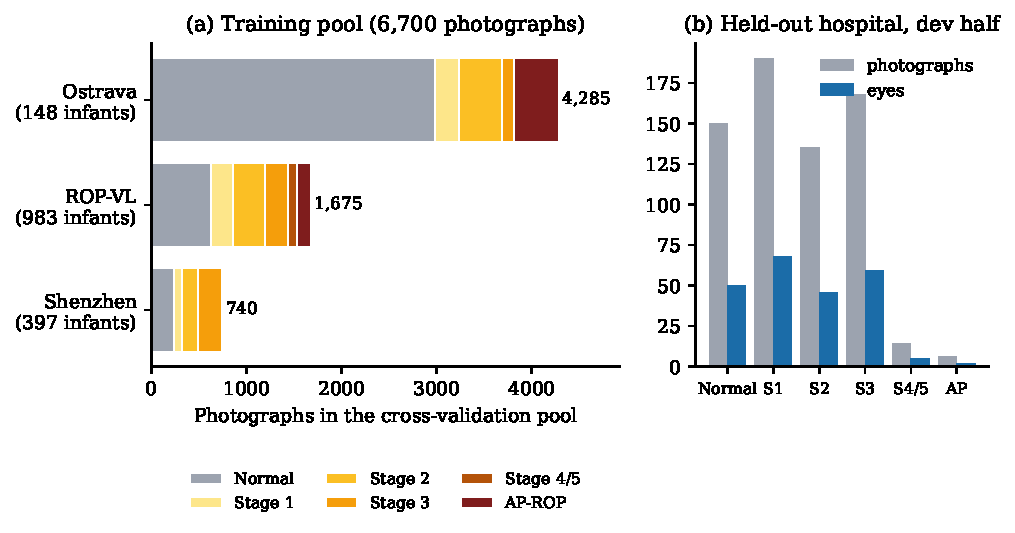
\includegraphics[width=\textwidth]{fig_dataset.pdf}
\caption{The data: (a) the cross-validation pool by hospital and stage; (b) the held-out hospital's development half, photographs and eyes by stage}\label{fig:dataset}
\end{figure}
\begin{table}[htbp]
\caption{Datasets, units and roles}\label{tab:data}
\begingroup\TightTable\small
\begin{tabularx}{\textwidth}{@{}p{24mm}p{20mm}p{18mm}Yp{30mm}@{}}\toprule
Cohort & Photographs & Infants & Label unit (scored at) & Role\\\midrule
Ostrava & 4{,}285 & 148 & examination session (both eyes) & CV pool\\
ROP-VL & 1{,}675 & 983 & photograph; eye-examination unit & CV pool\\
Shenzhen & 740 & 397 & photograph & CV pool; held out in the site fold\\
Multi-View, dev half & 663 (230 eyes) & 116 & eye (three views per eye) & held-out hospital, descriptive\\
Multi-View, locked half & 661 (230 eyes) & 116 & eye & pre-registered primary endpoint; unopened\\
\bottomrule\end{tabularx}\endgroup
\end{table}

The held-out hospital, Multi-View ROP, contributes to no fold and uses a different camera. Its 1{,}324 photographs are split by infant into a development half, used for the descriptive external results in this report, and a locked half opened once for the EfficientNet baseline in August 2026 and reserved for one further scoring of all arms after the guide's approval. The development half has 50 normal, 68 stage-1, 46 stage-2, 59 stage-3, 5 stage-4/5 and 2 AP-ROP eyes; the last two classes are too few to evaluate there.

Each training session trains on about 2{,}460 photographs (one fold's training rows after the caps and the duplicate exclusion) and is evaluated on the fold's 1{,}252--1{,}691 held-out photographs; the out-of-fold predictions of the five folds are concatenated to score the whole pool once, so every photograph is scored by a model that never saw its infant.

\section{Test Procedures and Repeated Trials}
Every trained arm was run twice end to end with different random seeds (42 and 1337), each run being five folds plus the site fold, giving 10 cross-validation models and 12 trained models per arm, 14 training sessions in the v3 round. The v4 round added models H and I (five folds, the site fold and two LOSO folds per seed, in two kernels per seed) and B's two LOSO folds (one kernel per seed): 10 further sessions, 24 in total. The learning rate for each transformer arm was chosen by a probe on an inner patient-disjoint split of fold~0's training rows (three candidates, one seed), never on fold~0's validation rows. Development-half predictions are made by all five fold checkpoints of each seed, giving 10 prediction lists per arm, whose metrics are averaged inside each bootstrap replicate. Each new model was first run for two epochs on the inner split as a smoke test (throughput, memory, no NaN, development scoring) before its full sessions were launched. Every kernel's log, summary and predictions were downloaded and checked by the collector; no run was discarded or re-run on the basis of its score.

\section{Performance Metrics and Analysis Method}
The primary metric is quadratic weighted kappa on the five-class map, with AP-ROP folded onto stage~4/5 on both sides,
\begin{equation}\label{eq:qwk}
\mathrm{QWK}=1-\frac{\sum_{i,j}w_{ij}O_{ij}}{\sum_{i,j}w_{ij}E_{ij}},\qquad w_{ij}=\frac{(i-j)^2}{(k-1)^2},
\end{equation}
where $O$ is the confusion matrix, $E$ its expectation under independence and $k=5$; a miss by two stages costs four times a miss by one. Secondary metrics are accuracy, balanced accuracy, macro-averaged precision, recall and F1 over the classes present, unweighted kappa, one-versus-rest AUC, any-ROP AUC and average precision, and per-class precision, recall and specificity. Calibration is reported as expected calibration error, Brier score and negative log-likelihood before and after one temperature $T$ fitted on cross-validation. The any-ROP operating point is the largest threshold on the eye's score $\max_i(1-p_{i,\text{normal}})$ that reaches 90\% sensitivity on cross-validation, applied unchanged at the new hospital.

Uncertainty: 95\% percentile intervals from 2{,}000 bootstrap resamples of infants; paired differences between arms are computed on the same resample and reported with their interval; an interval that crosses zero is read as no evidence of a difference. The selection rule, fixed in advance, is the cross-validation pooled out-of-fold image QWK, computed once per arm. The held-out hospital's development half is reported as descriptive because it was used for design decisions in the first version; model~F, which saw its photographs without labels, is marked as transductive. Failed trials are reported: the ordinal decoder's cross-validation drop and the adaptation model's closed confidence mask are both in Chapter~\ref{ch:results}.

\section{Fault Safety and Robustness Tests}
Software faults are covered by the test suite: malformed uploads, oversize requests, missing context, an unloaded model, misaligned predictions, a kernel that trained on excluded duplicates or at the wrong learning rate, a configuration that disagrees with its kernel, and any attempt to read the locked half. Robustness of the model was tested in four ways that the protocol allows: the site fold (Shenzhen held out entirely from training), the two further leave-one-source-out folds of the v4 round (Ostrava and ROP-VL held out in turn), the held-out hospital with a different camera, and the per-fold variability across the five folds and two seeds (Figure~\ref{fig:folds}). The operating threshold and the temperature were tested for transfer by applying the cross-validation values unchanged at the new hospital. No test was run on patients; the data are retrospective, public and de-identified.
